\chapter{Transverse Asymmetry}
The Beam Normal Single Spin Asymmetry (BNSSA, also known as Transverse Single Spin Asymmetry
or Transverse Asymmetry) is different from the PV asymmetry, it is purely 
electromagnetic and therefore parity-conserving. It arises from the interference
between one-photon and two-photon exchange (OPE and TPE), therefore it is sensitive 
to the TPE amplitude. By measuring it, we can probe the strength of TPE, an 
important knowledge of electron elastic scattering that may explain the myth
of proton radius measured with different methods.

The transver asymmetry is also an important systematic uncertainty to our PV 
asymmetry measurement, because there is always some residual transverse polarization
in the electron beam. With $\CA_n \sim \alpha_{EM}m_e/E_e$, its magnitude of $10^{-5}$
for a GeV level electron beam is much larger than $\CA_{pv}$, so a complete 
understanding and precise measurement of the transverse asymmetry is needed
to ensure accurate correction of $\CA_{pv}$.

Being a routine and bonus of a PV experiment, PREX-I also measured the transverse
asymmetry of some nuclei, namely ${}^{1}H$, \He, \C and \Pb. Surprisingly, PREX-I
saw a zero transverse asymmetry in \Pb, while the transverse asymmetries of other 
light nuclei seemed to agree with theoretical predications, as shown in 
Fig. \ref{fig:PREX-I_AT}. One of the reason for PREX-II was that we wanted to
verify the zero measurement in \Pb, which remains as a chanllenge to theorists.
\begin{figure}
    \centering
    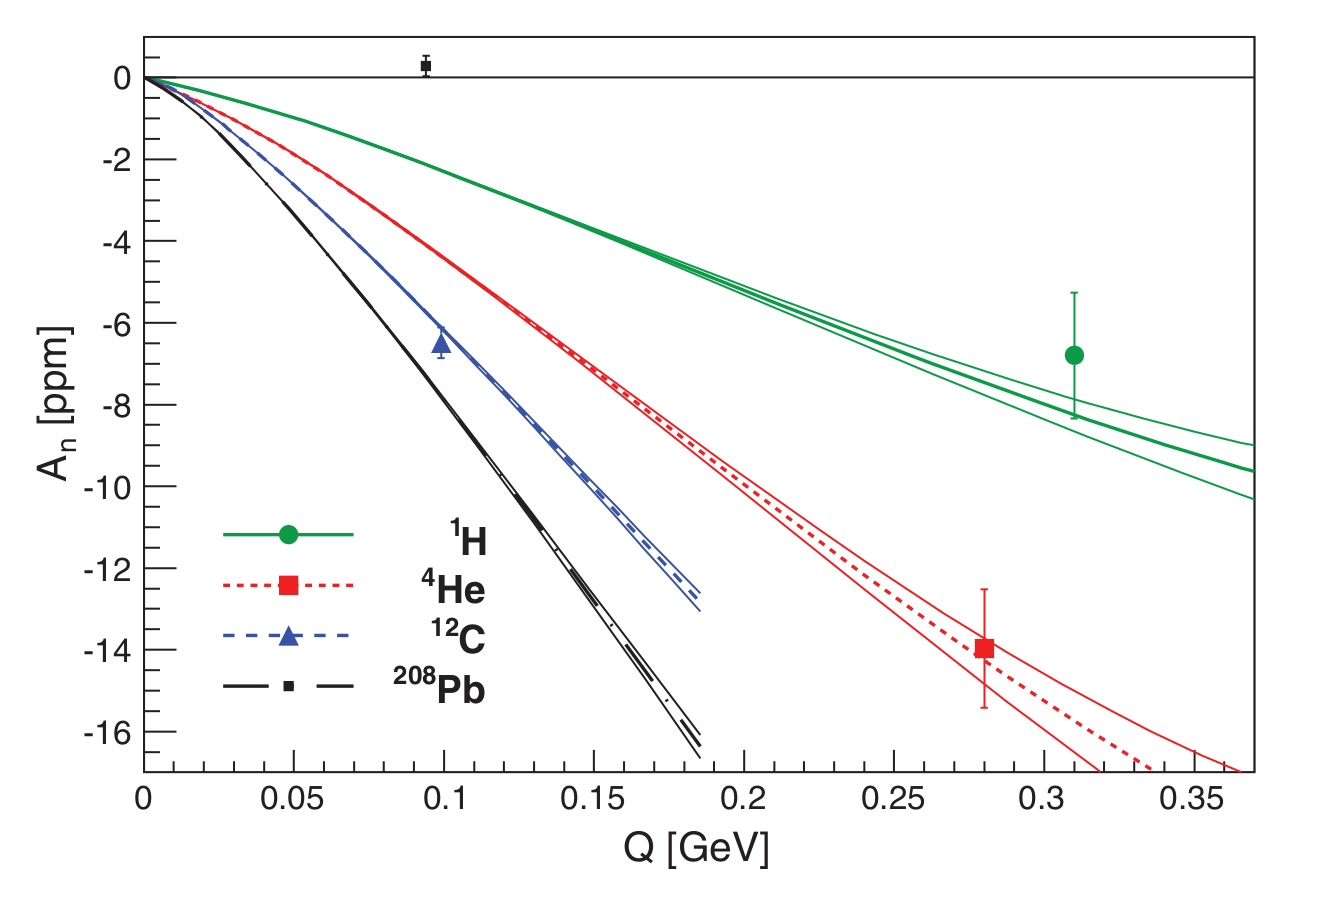
\includegraphics[width=0.5\linewidth]{PREX-I_AT}
    \caption{Transverse asymmetry measured in PREX-I.}
    \label{fig:PREX-I_AT}
\end{figure}

As its name implies, BNSSA depends on only one spin, either the target or the
electron, polarized target is better that polarized target in that it is hard
to polarize nuclei, especially heavy nuclei.

%%%%%%%%%%%%%%%%%%%%%%%%%%%%%%%%%%%%%%%%%%%%%%%%%%%%%%%%%%%%%%%%%%%%%%%%
\section{Motivation for Transverse Asymmetry}

%%%%%%%%%%%%%%%%%%%%%%%%
\subsubsection{The Scattering Theory}
Consider the scattering of a free ($t_0 \rightarrow -\infty$) particle from a 
time independent potential $V(\vec{r})$, 
which decays quickly as $r \rightarrow \infty$. The evolution from the free initial state
$\ket{i}$ is denoted as $\ket{\psi(t)}_S$ (under the Schr\"odinger picture, $\hbar = 1$):
\begin{equation}
    \ket{\psi(t)}_S = U(t)\ket{\psi(t_0)} = \lim_{t_0 \rightarrow -\infty}U(t, t_0)\ket{i}
\end{equation}
where $U(t, t_0)$ is the evolution operator:
\begin{equation}
    U(t, t_0) = \exp(\frac{1}{i}(H_0 + V)(t - t_0)) = \exp(-i(H_0 + V)(t-t_0))
\end{equation}
$H_0$ is the free Hamiltonian and $H = H_0 + V$ is the complete Hamiltonian
with interaction term. 

The projection of $\psi(t)$ to a free final state $\ket{f}$ defines the so called
S-matrix (the order of the subscripts matters):
\begin{equation}
    S_{if} \equiv \lim_{t\rightarrow +\infty}\bra{f}\ket{\psi(t)} 
    = \lim_{t\rightarrow\infty} \lim_{t_0 \rightarrow -\infty} \bra{f} U(t, t_0) \ket{i}
\end{equation}
Which defines the S operator:
\begin{equation}
    S_{if} = \bra{f} S \ket{i} \Longrightarrow S = U(+\infty, -\infty)
\end{equation}

The S-matrix describe the scattering amplitude from the free inital state $\ket{i}$
to the free final state $\ket{f}$. Conservation of probability indicates
unitary of S matrix:
\begin{equation}
    S^\dag S = \sum_f |\bra{f} U(+\infty, -\infty) \ket{i}|^2 = 1
\end{equation}

It is easier to evaluate $U(t)$ in the interaction picture. Define
\begin{equation}
    \ket{\psi(t)}_I \equiv \exp(-\frac{1}{i}H_0 t) \ket{\psi(t)}_S 
    = \exp(iH_0 t) \exp(-i (H_0 + V) t)\ket{i}
\end{equation}
The subscript I and S denote the interaction and Schr\"odinger picture respectively.
The evolution of $\ket{\psi(t)}_I$ is:
\begin{equation}
    \begin{aligned}
	\frac{d}{dt}\ket{\psi(t)}_I 
	&= \left[ \exp(i H_0 t) (iH_0) \exp(-i (H_0 + V) t)
	+ \exp(i H_0 t) (-i)(H_0 + V) \exp(-i (H_0 + V) t) \right] \ \ket{i}  \\
	&= -i\ \exp(i H_0 t)\ V \ \exp(-i (H_0 + V) t) \ket{i}   \\
	&= -i \exp(iH_0 t) V \exp(-iH_0 t) \cdot \exp(iH_0 t) \exp(-i(H_0 + V)t) \ket{i}   \\
	&= -i V_I(t) \ket{\psi(t)}_I
    \end{aligned}
    \label{eq:interaction_evolution}
\end{equation}
where $V_I(t) = \exp(iH_0t)V\exp(-iH_0t)$ is the time dependent interaction term.
Eq. \ref{eq:interaction_evolution} leads to the Dyson series:
\begin{equation}
    U(t, t_0) = 1 - i\int_{t_0}^t dt_1 V_I(t_1) U(t_1, t_0) = \sum_{n=0}^\infty \frac{(-i)^n}{n!}\int_{t_0}^t dt_1 \cdots \int_{t_0}^t dt_n T[V_I(t_1)\cdots V_I(t_n)]
\end{equation}
T means time-ordering:
\begin{equation}
    T(V_I(t_1) V_I(t_2)) \equiv 
    \begin{cases}
	V_I(t_1)V_I(t_2)    & t_1 \le t_2   \\
	V_I(t_2)V_I(t_1)    & t_2 \le t_1   \\
    \end{cases}
\end{equation}

\begin{equation}
    \begin{aligned}
	\bra{f} U(t, t_0) \ket{i} 
	&= \bra{f}\ket{i} - i \bra{f} \int_{t_0}^t dt_1 V_I(t_1) U(t_1, t_0) \ket{i}	\\
	&= \delta_{if} - i\sum_m \int_{t_0}^t dt_1 \bra{f}\exp(iH_0 t_1) V \exp(-iH_0 t_1)(t_1)\ket{m} \bra{m} U(t_1, t_0) \ket{i} \\
	&= \delta_{if} - i\sum_m \bra{f}V\ket{m} \int_{t_0}^t dt_1 \exp(i(E_f - E_m)t_1) \bra{m}U(t_1, t_0)\ket{i}  \\
    \end{aligned}
    \label{eq:finite_S-matrix}
\end{equation}
Truncate Eq. \ref{eq:finite_S-matrix} into first order ($\bra{m} U(t_1, t_0) \ket{i} = \delta_{im}$)
and define $T_{if} = \bra{f} V \ket{i}$, we will get:
\begin{equation}
    \bra{f} U(t, t_0) \ket{i} = \delta_{if} - iT_{if} \int_{t_0}^t dt_1 \exp(i(E_f - E_i)t_1)
\end{equation}
and 
\begin{equation}
    \begin{aligned}
	S_{if} &= \lim_{t\rightarrow +\infty}\lim_{t_0 \rightarrow -\infty} \bra{f} U(t, t_0) \ket{i}    \\
	    &= \delta_{if} - iT_{if} \int_{-\infty}^{\infty} dt_1 \exp(i(E_f - E_i)t_1)	\\
	    &= \delta_{if} + i2\pi\delta(E_f - E_i)T_{if}   \\
    \end{aligned}
\end{equation}
In matrix form:
\begin{equation}
    S = 1 + i2\pi T
\end{equation}
S begin unitary implies
\begin{equation}
    S^\dag S = (1 - i2\pi T^\dag) (1 + i2\pi T) = 1 + i2\pi(T - T^\dag) + (2\pi)^2 T^\dag T = 1
\end{equation}
which reads
\begin{equation}
    T - T^\dag = i (2\pi)T^\dag T = i(2\pi) T T^\dag
\end{equation}
In terms of matrix element:
\begin{equation}
    \begin{gathered}
    \delta(E_f - E_i)(T_{if} - T^\dag_{if}) = \sum_m i2\pi\delta(E_f - E_m)\delta(E_m - E_i)T_{fm}T^\dag_{mi}	\\
    T_{if} - T^\dag_{if} = \sum_m i2\pi\delta(E_m - E_i)T_{fm}T^\dag_{mi} = ia_{if} \\
    \end{gathered}
\end{equation}
where 
\begin{equation}
    a_{if} = \sum_m (2\pi) \delta(E_m - E_i)T_{fm}T^\dag_{mi}
\end{equation}
is the absorptive part of the transition amplitude $T_{if}$. $\ket{m}$ extends
to all on-shell intermediate states.

The two parts of S are easy to understand.
The constant piece denotes the evolution of one free particle into another free
particle without any interactions; obviously, it can evolve only into itself.
The T matirx describe the interaction (transition amplitude) between the free
initial particle $\ket{i}$ and the free final particle $\ket{j}$, which tells
us the interaction cross section.

The free particle state can be completely described by its momentum (ignoring spin
for now) $\vec{p}$. For an incoming electron $\ket{\vec{p}_i}$, the probability
to transform into the final state of $\ket{\vec{p}_f}$ is:
\begin{equation}
    dP = (phase\ space) \times (transition\ probability) = \frac{d\vec{p}_f}{(2\pi)^3} \times |S_{\vec{p}_i\vec{p}_f}|^2
\end{equation}
For a non trivial case of $\ket{f} \ne \ket{i}$, we have:
\begin{equation}
    S_{if} = i2\pi \delta(E_f - E_i)T_{if}
\end{equation}
The differential cross section will be:
\begin{equation}
    d\sigma = \frac{dP}{\CL \Delta t}
\end{equation}
where $\CL$ is the luminosity, indicating number of particles hitting 
the target per unit area per unit time, in our case of incoming plane wave, 
$\CL = \rho v = v$, and $\Delta t$ is the interaction time.
\begin{equation}
    d\sigma = \frac{1}{v\Delta t} \frac{d\vec{p}_f}{(2\pi)^3} 2\pi\delta(E_f - E_i) \left. 2\pi\delta(E_f - E_i)\right|_{E_f = E_i} |T_{if}|^2
\end{equation}
Transform one $\delta$ back to integrating form: 
\begin{equation}
    \left. 2\pi\delta(E_f - E_i) \right|_{E_f = E_i} 
    = \int_{-\infty}^{+\infty} dt \left.\exp(-i(E_f - E_i)t)\right|_{E_f = E_i}
    = \int_{-\infty}^{+\infty} dt 
\end{equation}
Physically, we don't go back or into infinity in time, because the real particle
is a finite wave packet rather than a plane wave. The integration above should 
be finite and close to the interaction time
\begin{equation}
    \int_{-\infty}^{+\infty} dt \rightarrow \Delta t
\end{equation}
Thus we have a defined cross section
\begin{equation}
    d\sigma = \frac{1}{v} \frac{d\vec{p}_f}{(2\pi)^3} 2\pi\delta(E_f - E_i) |T_{if}|^2
\end{equation}
The cross section is proprotianal to $|T_{if}|^2$, as known to us.


%%%%%%%%%%%%%%%%%%%%%%%%
\subsubsection{T-Symmetry}
Symmetry is the most profound concept and foundation of modern physics, which
can be seperated into continuous symmetries and discrete ones. Time symmetry
is one important discrete symmetry, which states that physical laws should
keep unchange under time reversal operation. Time reversal is the operation
that flips time arrow, so that time runs backward after time reversal. Obviously, 
vectors that are first order of time derivative will also reverse sign, such
as momentum, angular momentum and magnetic field.

Express the time reversal operation in QM:
\begin{equation}
    \ket{\tilde{\psi}} = \hat{\mathcal{T}} \ket{\psi} 
\end{equation}
where $\hat{\mathcal{T}}: t \rightarrow -t$ is the time reversal operator. 

In terms of our scattering, as said above, a particle will flip its momentum 
and spin (angular momentum) under time reversal, and pick up a phase.
\begin{equation}
    \ket{\tilde{\psi}} = \hat{\mathcal{T}} \ket{\psi_\uparrow(\vec{k})} = \eta\ket{\psi_\downarrow(-\vec{k})}
\end{equation}
$\eta$ is the phase difference, $|\eta|^2 = 1$. So the T matrix can also be applied
to time reversed state
\begin{equation}
    T_{\tilde{i}\tilde{f}} = \bra{\tilde{f}} V \ket{\tilde{i}}
\end{equation}

It is well known that electromagnetic interaction is invariant under time reversal.
\begin{equation}
    |T_{if}|^2 = |T_{\tilde{f}\tilde{i}}|^2 
\end{equation}

With these concepts, one can also define the \textbf{T-odd} quantities which
are proportional to the difference of the magnitude of a normal T element and 
its half time reversed version:
\begin{equation}
    \begin{aligned}
	\text{T-odd} &\propto |T_{if}|^2 - |T_{\tilde{i}\tilde{f}}|^2	\\
	    &= |T_{if}|^2 - |T_{fi}|^2	\\
	    &= |T_{if}|^2 - |T^\dag_{if}|^2	\\
	    &= |T_{if}|^2 - |T_{if} - ia_{if}|^2	\\
	    &= -i(T_{if}a^*_{if} - T^*_{if}a_{if}) - |a_{if}|^2	\\
	    &= 2Im(T_{if}a^*_{if}) - |a_{if}|^2
    \end{aligned}
    \label{eq:T-odd}
\end{equation}

%%%%%%%%%%%%%%%%%%%%%%%%
\subsubsection{Transverse Asymmetry}
Denote the incoming and outgoing transversely polarized electrons as 
$\ket{\vec{k}}$ and $\ket{\vec{k}'}$, the scattering is shown in Fig. \ref{fig:transverse_scattering}.
\begin{figure}[h!]
    \centering
    \begin{subfigure}[c]{0.4\linewidth}
	\begin{tikzpicture}[scale=0.8]
	    \begin{feynman}[transform shape]
		\vertex (i1) {$e^-$};
		\vertex [right=1.0cm of i1, inner sep=0pt] (spin) {$\odot$};
		\vertex [right=2.3cm of spin] (ip);
		\vertex [right=2.8cm of ip] (i2) {A};
		\vertex [above right = 2cm and 2cm of ip] (o1) {$e^-$};
		\vertex [below left = 2cm and 2cm of ip] (o2) {A};

		\diagram* { {[edge=fermion]
		    (spin) --[edge label=$\vec{k}$] (ip) [dot] --[edge label = $\vec{k}'$] (o1),
		    (i2) --[edge label=$\vec{p}$](ip) [dot] -- [edge label = $\vec{p}'$]  (o2)},
		    (i1) -- (spin)
		};
	    \end{feynman}
	\end{tikzpicture}
    \end{subfigure}
    \hspace{0.2 cm}
    \textbf{-}
    \hspace{0.5 cm}
    \begin{subfigure}[c]{0.4\linewidth}
	\begin{tikzpicture}[scale=0.8]
	    \begin{feynman}[transform shape]
		\vertex (i1) {$e^-$};
		\vertex [right=1.0cm of i1, inner sep=0pt] (spin) {$\otimes$};
		\vertex [right=2.3cm of spin] (ip);
		\vertex [right=2.8cm of ip] (i2) {A};
		\vertex [above right = 2cm and 2cm of ip] (o1) {$e^-$};
		\vertex [below left = 2cm and 2cm of ip] (o2) {A};

		\diagram* { {[edge=fermion]
		    (spin) --[edge label=$\vec{k}$] (ip) [dot] --[edge label = $\vec{k}'$] (o1),
		    (i2) --[edge label=$\vec{p}$](ip) [dot] -- [edge label = $\vec{p}'$]  (o2)},
		    (i1) -- (spin)
		};
	    \end{feynman}
	\end{tikzpicture}
    \end{subfigure}
    \caption{Feynman plots of transversely polarized electron scatters off
    unpolarized nuclear target in the CoM. } 
    \label{fig:transverse_scattering}
\end{figure}

The transverse asymmetry will be:
\begin{equation}
    \CA_n \equiv \frac{N_{\uparrow} - N_{\downarrow}}{N_{\uparrow} + N_{\downarrow}} 
    = \frac{|T_{\uparrow}(\vec{k}, \vec{k}')|^2 - |T_{\downarrow}(\vec{k}, \vec{k}')|^2}{|T_{\uparrow}(\vec{k}, \vec{k}')|^2 + |T_{\downarrow}(\vec{k}, \vec{k}')|^2}
\end{equation}
where $T(\vec{k}, \vec{k}') = \bra{\vec{k}'} V \ket{\vec{k}}$ is the scattering
amplitude and the arrow subscript indicates electron's spin direction.
$T_\downarrow(\vec{k}, \vec{k}')$ is related to $T_\downarrow(-\vec{k}, -\vec{k}')$
by a rotation around the normal direction of the scattering plane, as shown in
Fig. \ref{fig:rotation_plot}
\begin{figure}[h!]
    \centering
    \begin{subfigure}[c]{0.4\linewidth}
	\begin{tikzpicture}[scale=0.8]
	    \begin{feynman}[transform shape]
		\vertex (i1) {$e^-$};
		\vertex [right=1.0cm of i1, inner sep=0pt] (spin) {$\odot$};
		\vertex [right=2.3cm of spin] (ip);
		\vertex [right=2.8cm of ip] (i2) {A};
		\vertex [above right = 2cm and 2cm of ip] (o1) {$e^-$};
		\vertex [below left = 2cm and 2cm of ip] (o2) {A};

		\diagram* { {[edge=fermion]
		    (spin) --[edge label=$\vec{k}$] (ip) [dot] --[edge label = $\vec{k}'$] (o1),
		    (i2) --[edge label=$\vec{p}$](ip) [dot] -- [edge label = $\vec{p}'$]  (o2)},
		    (i1) -- (spin)
		};
	    \end{feynman}
	\end{tikzpicture}
    \end{subfigure}
    \hspace{0.2 cm}
    $\Longrightarrow$
    \hspace{0.5 cm}
    \begin{subfigure}[c]{0.4\linewidth}
	\begin{tikzpicture}[scale=0.8]
	    \begin{feynman}[transform shape]
		\vertex (i1) {$e^-$};
		\vertex [left=1.0cm of i1, inner sep=0pt] (spin) {$\odot$};
		\vertex [left=2.3cm of spin] (ip);
		\vertex [left=2.8cm of ip] (i2) {A};
		\vertex [below left = 2cm and 2cm of ip] (o1) {$e^-$};
		\vertex [above right = 2cm and 2cm of ip] (o2) {A};

		\diagram* { {[edge=fermion]
		    (spin) --[edge label=$\vec{k}$] (ip) [dot] --[edge label = $\vec{k}'$] (o1),
		    (i2) --[edge label=$\vec{p}$] (ip) [dot] -- [edge label = $\vec{p}'$] (o2)},
		    (i1) -- (spin)
		};
	    \end{feynman}
	\end{tikzpicture}
    \end{subfigure}
    \caption{Rotation by $\pi$ around the normal direction.} 
    \label{fig:rotation_plot}
\end{figure}
\begin{equation}
    T_\downarrow(\vec{k}, \vec{k}') = e^{i\pi} T_\downarrow(-\vec{k}, -\vec{k}')
\end{equation}

Let $T_{if} = T_{\uparrow}(\vec{k}, \vec{k}')$, then $T_{\tilde{i}\tilde{f}} = T_\downarrow (-\vec{k}, -\vec{k}')$
and
\begin{equation}
    \begin{aligned}
	\CA_n &\approx \frac{|T_{\uparrow}(\vec{k}, \vec{k}')|^2 - |T_{\downarrow}(-\vec{k}, -\vec{k}')|^2}{2|T_{\uparrow}(\vec{k}, \vec{k}')|^2} \\
	    &= \frac{|T_{if}|^2 - |T_{\tilde{i}\tilde{f}}|^2}{2|T_{if}|^2}  \\
	    &= \frac{2Im(T_{if}a^*_{if}) - |a_{if}|^2}{2|T_{if}|^2}
    \end{aligned}
    \label{eq:transverse_asymmetry}
\end{equation}

We see that the transverse asymmetry is a T-odd quantity. For EM interaction
\begin{equation}
    T_{if} \propto \alpha \qquad a_{if} \propto \alpha^2
\end{equation}
Because $\alpha \simeq \frac{1}{137}$ is small, we can expand Eq. \ref{eq:transverse_asymmetry} 
in order of $\alpha$. To the lowest order
\begin{equation}
    \CA_n = 0
    \label{eq:AT_0}
\end{equation}
and to the first order 
\begin{equation}
    \CA_n = \frac{Im(T_{if}a^*_{if})}{|T_{if}|^2}
    \label{eq:AT_1}
\end{equation}

$T_{ij}$ represents the OPE interaction while $a_{ij}$ represents
the TPE interaction. So the physical interpreation of
Eq. \ref{eq:AT_0} and \ref{eq:AT_1} is that time reversal symmetry requires 
the transverse asymmetry to be zero under the Born approximation (OPE only)
and the (lowest order) non-zero transverse asymmetry comes from the interference 
between OPE and TPE.
\begin{figure}[h!]
    \centering
    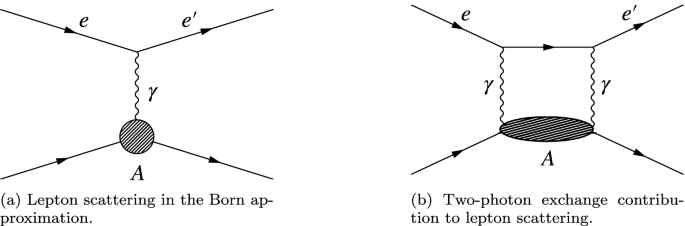
\includegraphics[width=0.8\linewidth]{OPE_n_TPE}
\end{figure}

%%%%%%%%%%%%%%%%%%%%%%%%%%%%%%%%%%%%%%%%%%%%%%%%%%%%%%%%%%%%%%%%%%%%%%%%
\section{How to Measure the Transverse Asymmetry: the Method}
The experimentally measured transverse asymmetry will be
\begin{equation}
    \CA_{mea} = \CA_n \vec{p}_e \cdot \hat{n} = \CA_n |p_e| \sin(\phi_s - \phi_e)
\end{equation}
where $\vec{p}_e$ is the electron spin direction and $\phi_s$ being its angle
w.r.t. the lab horizontal plane; $\hat{n} = \frac{\vec{k}' \times \vec{k}}{|\vec{k}' \times \vec{k}}$ 
is the unit normal vector of the scattering plane and $\phi_e$ the angle between
the scattering plane and the lab horizontal plane. As shown in Fig. \ref{fig:AT_scattering}..
\begin{figure}[h!]
    \centering
    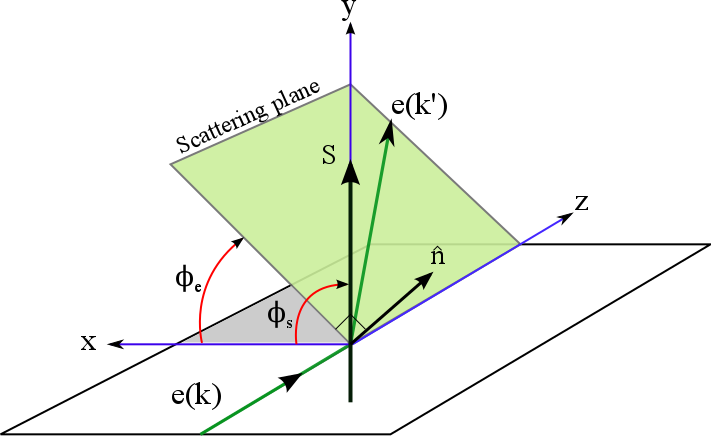
\includegraphics[width=0.7\linewidth]{AT_scattering}
    \caption{Schematic plot of transverse scattering.}
    \label{fig:AT_scattering}
\end{figure}
We see an angle dependence of the measured transverse asymmetry. Experimentally,
it is convenient to select the angle $\phi_s - \phi_e$ being $90^\circ$, which
usually set the lab horizontal plane as the scattering plane and the electron spin
is perpendicular to the scattering plane, as we did in PREX-II and CREX. 

To achieve transverse polarization, we needed a different configuration of the
double wien filter. Specifically, we just rotated the longitudinal spin originated
from the source to vertically direction using the vertical wien filter, the 
following rotation we did for longitudinal polarization, as shown in 
Fig. \ref{fig:double_wien_filter}, was omitted. Because the spin is parallel/anti-parallel
to the magnetic field in the accelerator arc, there is no spin precession as in
the case of longitudinal polarization. 

% how much data is needed?
% polarization measurement
Except the difference in configuration of the double wien filter, everything 
else was the same as in the case of longitudinal polarization. We spent 

%%%%%%%%%%%%%%%%%%%%%%%%%%%%%%%%%%%%%%%%%%%%%%%%%%%%%%%%%%%%%%%%%%%%%%%%
\section{The Result}

